\documentclass[12pt, a4paper]{article} 
\usepackage{eurosym}  
\usepackage[margin = 1.2in]{geometry}
\usepackage[french]{babel}
\usepackage[utf8x]{inputenc}
\usepackage{graphicx}
\usepackage[T1]{fontenc}
\usepackage{fancyhdr}
\usepackage{hyperref}
\pagestyle{fancy}
\setlength{\headheight}{15pt}
\fancyhead[L]{SharpBoy}
\fancyhead[R]{EPITA}
\fancyhead[C]{S\_Society}
\renewcommand{\footrulewidth}{1pt} 
\fancyfoot[L]{Rapport de soutenance 1}
\fancyfoot[R]{2016-2017}
\fancyfoot[C]{\thepage}
\title{\Huge \bf SharpBoy}
\author{\LARGE \bf S\_Society }
\title{\Large \bf Rapport de Soutenance}


\begin{document}


\maketitle


\bigskip
\large Gabriel DUQUE: duque\_g

\bigskip
\large Antoine MARTIN: ma\_9

\bigskip
\large Martin MEUNIER : meunie\_o

\bigskip
\large Ilyes NOUMRI : noumri\_i

\bigskip
\large {\textbf{Projet S2\#}}

\bigskip 
\bigskip
\bigskip



\begin{center}

\includegraphics[width= 12cm]{logo-epita-hd.png} 
\end{center}


\pagebreak

\tableofcontents 

\pagebreak

\large
\section{Introduction}
Après la validation du cahier des charges, le groupe a directement commencé à étudier les spécificités du F\# qui est un nouveau langage pour nous. Notre projet étant assez complexe pour notre niveau, nous avons commencé par nous atteler à un sous-projet nous permettant de comprendre comment fonctionne l'émulation en général. C'est la raison pour laquelle nous avons décidé de réaliser un émulateur Chip-8 dans un premier temps.

\medskip
Le Chip-8 est un langage de programmation hexadécimal qui sera interprété en utilisant une machine virtuelle. Il a été conçu pour faciliter la conception de jeux-vidéos sur les micros-ordinateur 8-bits. Celui-ci nous permettra de comprendre comment un émulateur est structuré. 

\medskip
Notre objectif pour cette première soutenance était donc d'acquérir de nouvelles connaissances sur l'émulation en général et sur les spécificités du F\# et de se lancer dans le début de la SharpBoy.

\bigskip
\bigskip
\begin{center}
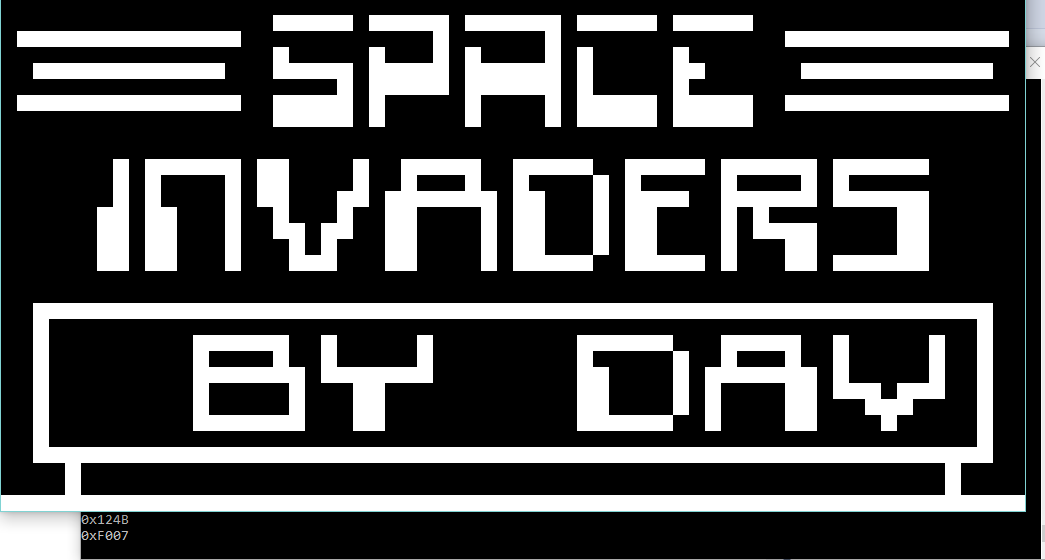
\includegraphics[width=14cm]{chip8cap3.PNG}
\end{center}

\pagebreak

\section{Retour sur le cahier des charges}
\subsection{Équipe}
L'équipe n'a pas changé et est toujours aussi motivée pour mener le projet à bien. Elle est constituée de Gabriel DUQUE, Antoine MARTIN, Martin MEUNIER, Ilyes NOUMRI.
\subsection{Objectif final}
L'objectif final est de réaliser un émulateur GameBoy fonctionnel et complet. Cela nous permettra d'avoir des connaissances sur le fonctionnement d'un processeur et d'un système en général pour la suite de nos études. 

De plus, l'apprentissage d'un nouveau langage, en l'occurrence le F\# ne peut être que bénéfique pour la suite de nos études et pour notre compréhension des concepts d'algorithmique théorique.
\bigskip
\subsection{Répartition des tâches}
\bigskip
\bigskip


\begin{center}
\begin{tabular}{|l|c|c|c|c|}
\hline
\bf Tâches                & \bf Gabriel   & \bf Antoine   & \bf Martin    & \bf Ilyes\\
\hline 
Menus/Options       &      x       &               &         x     &       \\
\hline 
Site web            &               &         x     &               &     x  \\
\hline 
Vidéo               &          x    &               &       x       &       \\
\hline 
CPU                 & x             & x             &               &       \\
\hline 
Mémoire             &               & x             &               &  x \\
\hline
Audio               &               &               & x             & x \\
\hline
Marketing           & x             &               &               & x \\
\hline
Réseau              &               &               & x             & x \\ 
\hline
\end{tabular}
\end{center}
\bigskip
\pagebreak

\section{Avancement du projet}
\subsection {Les préliminaires}
\subsubsection {\large Une expérience nécessaire}  
Avant de nous attaquer à la programmation d'une GameBoy en ne partant de rien nous avons jugé judicieux de commencer par émuler une console plus ancienne et donc a fortiori moins complexe. Après une recherche productive, nous avons décidé de nous pencher sur le Chip-8 qui était un langage interprété qui tournait dans une machine virtuelle. Il était utilisé sur des micros-ordinateurs 8-bit comme le COSMAC VIP ou encore le Telmac 1800.

Ce langage date de 1978 et l'émulation de son fonctionnement est considérée comme une phase préliminaire à l'émulation de machines plus récentes. Les intérêts de cette étape sont nombreux. Premièrement, une compréhension profonde du fonctionnement d'une machine est indispensable pour réaliser la SharpBoy. Comprendre la manière dont la mémoire et les registres sont gérés sur un modèle simple nous a grandement aidé pour notre compréhension de la GameBoy. 

Par la suite, l'implémentation des instructions en F\# a été également très didactique pour la SharpBoy car encore une fois, la GameBoy suit en fait le même modèle que le Chip-8 mais en plus poussé et complexe.

\subsubsection{\large Le F\#}
Avant de commencer à coder, notre groupe a été confronté à un problème d'ordre pratique: apprendre le F\#. Ayant décidé de réaliser notre projet dans ce langage fonctionnel qui nous était inconnu à l'époque, nous avons fait plusieurs tutoriels sur internet pour nous familiariser avec sa syntaxe nouvelle mais en même temps assez familière car il dérive de deux langages que nous connaissons.

Pour mesurer nos acquis, nous avons recodé certaines fonctions de base comme fibo et factorielle en F\# pour être sûrs de tous être à jour pour ne pas foncer droit dans le mur et tout coder à l'aveugle.
\pagebreak 

\subsubsection {\large Un GitHub rigoureux}
Les membres de S\_Society ont décidé d'utiliser Git pour partager notre code. Nous utilisons Git à travers la plateforme GitHub pour avoir accès à nos fichiers à distance et pouvoir les modifier depuis n'importe où.

\bigskip
De plus, nous avons paramétré le dépôt de manière à pouvoir travailler en équipe et ne pas avancer en excluant un membre. Plusieurs mesures on étés prises pour éviter de laisser tomber un membre au fur et à mesure que le projet avance et que le code à produire devient de plus en plus complexe. 

\bigskip
Premièrement, nous avons bloqué le push (l'ajout de lignes de code à un fichier) directement dans la branche master (branche principale) pour éviter de devoir revenir en arrière. Chaque membre crée donc des branches différentes pour ajouter son code puis les branches sont fusionnées avec master plus tard lorsque leur code est définitif. 

\bigskip
Deuxièmement, nous avons utilisé le système de code review (relecture de code) proposé par GitHub afin de bloquer la fusion de branches jusqu'à ce que le code soit approuvé par l'ensemble des membres du groupe. Cette dernière mesure force tout le monde à lire le code des autres membres afin de vérifier que tout le monde comprend le code des autres avant de fusionner définitivement les branches.

\bigskip
Ces mesures combinées assurent une progression commune des \linebreak membres du groupe afin de s'assurer que tout le monde comprend bien le code et progresse individuellement dans tous les domaines de la programmation auxquels touche notre projet.

\pagebreak

\subsection {Un Chip-8 fonctionnel}
Comme dit ci-dessus, nous avons implémenté un Chip-8 en F\#. Cette tâche a occupé la majorité du temps précédent cette première soutenance.

\subsubsection{\large Structure}
La structure de notre programme a été pensée par tous pour que notre programme soit organisé de manière cohérente. Nous avons séparé notre programme en 3 modules distincts : un module contenant les instructions du processeur, un module contenant les implémentations de la mémoire, des touches et des informations concernant l'affichage et enfin un module programme qui contient la boucle principale qui fera tourner notre programme et les informations sur la fenêtre de lancement ainsi que des éléments du débogage.

\subsubsection{\large CPU}
Il y a 34 instructions pour le processeur donc nous nous sommes réparti les instructions en expliquant clairement à nos camarades ce que notre code fait. Une instruction est composé de 4 chiffres hexadécimaux : un premier chiffre qui sert à identifier l'instruction suivi des paramètres de l'instruction. 

Gabriel s'est occupé par exemple de l'instruction appelé CXKK qui consiste à affecter le résultat d'une opération de bits (en l'occurrence un AND) entre la valeur KK et un nombre aléatoire au registre VX.

Antoine s'est occupé par exemple de l'instruction appelée FX33 qui consiste à stocker la représentation BCD (binary coded decimal) du registre VX à l'adresse mémoire I,  I+1, I+2

Martin lui s'est occupé par exemple de l'instruction 5XY0 qui passe à l'instruction suivante si le registre VX est égal à l'adresse Y dans ce même registre.

Ilyes s'est occupé par exemple de l'instruction DXYK qui dessine un sprite en X,Y de hauteur K et de longueur 8. 

\pagebreak

\subsubsection{\large Boucle principale et affichage}
La boucle principale implémentée dans le fichier Program.fs constitue les rails de l'émulateur. Concrètement,
elle consiste en un lancement de l'émulateur en chargeant une ROM et en démarrant une boucle qui continue tant qu'il y a des instructions à lire. De plus, cette fonction gère aussi la synchronisation des évènements en traitant une instruction toutes les millisecondes pour assurer une fluidité de jeu sans alourdir trop la complexité de l'algorithme avec des tests trop fréquents.

Le fichier Program.fs gère aussi l'affichage des différentes fenêtres qui, elles, sont soit des Windows Forms soit la console. Le dialogue initial permet à l'utilisateur de choisir une ROM parmi ses fichiers et de charger cette dernière dans la mémoire. 

\bigskip
\subsubsection{\large Gestion des instructions et mémoire}
La gestion des instructions se fait dans la fonction main\_loop du fichier Program.fs. En effet, après avoir chargé la ROM, pour traiter les instructions ils sont tous passés un à un dans un pattern matching qui permet au programme d'appeler la bonne fonction et ainsi l'exécuter.

La mémoire, elle, est représentée par un tableau contenant 4096 cases car la Chip-8 a une mémoire de 4Mo et on peut ainsi stocker les données nécessaires au bon fonctionnement de l'émulateur.
\pagebreak
\subsection {Un début de SharpBoy}

\subsubsection{\large Des recherches bien avancées}
En ce qui concerne la GameBoy, notre première étape a été de lire de la documentation concernant cette console. Cette documentation nous a surtout servi à comprendre les différences entre la Chip-8 et la GameBoy. La documentation étant abondante sur internet dû à la popularité de la console, nous avons pu choisir les manuels du CPU qui nous semblaient les mieux expliqués et le plus exhaustif. Grâce à cette comparaison il a été plus facile pour nous de dégrossir le travail concernant la SharpBoy. 

Nous avons donc pu comprendre le fonctionnement de la GameBoy et commencer à mettre en place la structure principale de celui-ci dans les fichiers du code source du futur programme.

\subsubsection{\large Un squelette de code}
Dans la continuation d'une part de nos recherches et d'autre part de la Chip-8, nous avons créé les fichiers nécessaires pour la GameBoy et commencé à les remplir. 

En effet, nous avons déjà déclaré la majorité des variables qui nous seront nécessaires pour le projet. Les registres sont implémentés de même que la mémoire. Nous avons également créé la fonction concernant le dialogue avec l'utilisateur permettant à celui-ci de sélectionner une ROM et de la charger dans la mémoire.

\subsubsection{\large Un dépôt GitHub et un site mis à jour}

Pour bien se lancer dans la SharpBoy, nous avons créé un nouveau dépôt sur GitHub: Sharpboy ! Nous avons donc ajouté le squelette de code au dépôt et mis à jour notre fichier README pour garder une trace de notre progression. 

De plus, tout au long de la progression du Chip-8 nous avons postés des billets sur le site internet pour faire part au public de nos avancées et nos problèmes. Ainsi, notre site est aujourd'hui à jour par rapport à notre projet et on peut y trouver des liens vers nos dépôts GitHub et vers de la documentation.


\subsection{Site Web}
Bien que le site soit déjà créé et accessible, le temps que nous lui avons accordé pour l'instant est assez réduit. Néanmoins, nous avons posté quelques billets pour témoigner de la progression de la Chip-8 ainsi que du début de la SharpBoy. Ainsi, outre ces posts, nous avons implémenté la structure du site que nous compléterons au fur et à mesure de l'avancée du projet.

En outre, pour simplifier la publication sur le site internet qui est hébergé sur GitHub nous avons utilisé le générateur de site statique Jekyll pour automatiser la publication de billets en créant les fichiers des posts dans une branche dédiée (gh-pages) dans le dépôt SharpBoy.

\bigskip
\section{Planning}
\begin{center}
\begin{tabular}{|l|c|c|c|}
\hline
\bf Tâches          & \bf Soutenance 1      & \bf Soutenance 2      & \bf Soutenance 3  \\
\hline 
Menus/Options       &      0\%              &         0\%           & 100\%  \\
\hline 
Site web            &        66\%           &        100\%          & 100\%  \\
\hline 
Vidéo               &       33\%            &         66\%          & 100\%  \\
\hline 
CPU                 & 33\%                  &  66\%                 & 100\%  \\
\hline 
Mémoire             & 66\%                  & 100\%                 & 100\%  \\
\hline
Audio               &    0\%                & 33\%                  & 100\%  \\
\hline
Réseau              & 0\%                   & 25\%                  & 100\%  \\

\hline
\end{tabular}
\end{center}
\pagebreak
\section{Problèmes rencontrés pendant le projet}

Durant la création de le Chip-8 nous avons rencontré quelques difficultés au niveau du code et de son fonctionnement.

En effet, lors des phases de test des ROM de Chip-8, nous avons remarqué des erreurs ou des bugs nous empêchant de jouer et donc nous devions les corriger au plus vite. 

\bigskip
Pour cela, nous avons utilisé plusieurs méthodes pour résoudre ces erreurs. Tout d'abord, nous avons tous vérifié notre code pour potentiellement trouver la source du problème. Ensuite, nous avons testé notre émulateur en le comparant avec un autre émulateur en C qui fonctionne parfaitement pour trouver des erreurs visibles sur l'émulateur. Enfin, en ayant encore des erreurs après ces méthodes nous avons du tester ligne par ligne nos instructions en regardant par exemple les instructions utilisées dans le jeu pour nous concentrer sur celles-ci.

C'est avec plaisir que nous vous présentons notre émulateur qui ne possède plus aucun bug.

\bigskip
\begin{center}
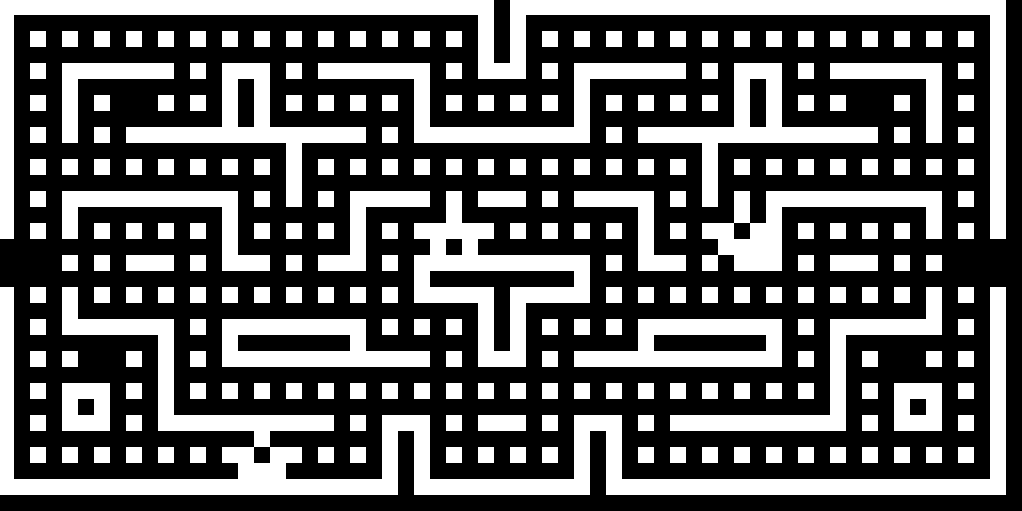
\includegraphics[width = 14.5cm]{chip8cap1.PNG}
\caption{Le jeu Blinky}
\end{center}
    




\pagebreak

\section{Tâches à effectuer pour la prochaine soutenance}

En ce qui concerne la prochaine soutenance, nous avons un planning plutôt ambitieux. En effet, nous avons prévu d'avoir un émulateur qui permettra de jouer à une ROM sans son et sans possibilité de sauvegarder une partie. Cette SharpBoy "brute" serait ensuite une base sur laquelle viendrait se greffer en vue de la troisième soutenance le son, les sauvegardes et potentiellement en fonction du temps restant, d'autres fonctionnalités.   

En vue d'aboutir le plus rapidement à un programme fonctionnel, nous avons décidé de ne pas implémenter le son ni la sauvegarde de parties pour cette soutenance. Le son étant sûrement l'attribut de la console le plus compliqué à émuler et n'étant pas essentiel pour une expérience de jeu convenable, il nous a semblé logique de laisser cet aspect de côté.

De plus, nous avons choisi de ne pas gérer le système de sauvegarde de parties pour les jeux. La raison nous poussant à faire ce choix est simple: notre priorité est d'avoir un émulateur qui marche pour pouvoir sereinement ajouter les fonctionnalités pour la soutenance finale.

Aussi, le site internet sera mis à jour de plus en plus régulièrement au fur et à mesure que l'on se rapproche du produit fini. Son aspect et son organisation seront revus pour le rendre plus intéressant et unique.

\pagebreak

\section{Bibliographie}
MSDN - Pour la documentation du F\#:

\url{https://msdn.microsoft.com/en-us/visualfsharpdocs/}

\url{conceptual/visual-fsharp-development-portal}

\bigskip
FSharp.org - Pour l'apprentissage du F\#:

\url{http://fsharp.org/}

\bigskip
FSharp For Fun and Profit:

\url{http://fsharpforfunandprofit.com}

\bigskip
Page Wikipedia du Chip-8:  

\url{https://en.wikipedia.org/wiki/CHIP-8}

\bigskip
Documentation technique du Chip-8:  

\url{http://devernay.free.fr/hacks/chip8/C8TECH10.HTM}

\bigskip
CodeSlinger.co.uk - Un site où est réuni de la documentation

technique sur la chip-8, un guide d'instruction, ainsi que le code

d'un émulateur complet en C:

\url{http://www.codeslinger.co.uk}

\bigskip

Page Wikipedia de la GameBoy:

\url{https://en.wikipedia.org/wiki/Game_Boy}

\bigskip

Documentation technique de la GameBoy:

\url{http://marc.rawer.de/Gameboy/Docs/GBCPUman.pdf}

\bigskip
Tableau des instructions pour la GameBoy:

\url{http://pastraiser.com/cpu/gameboy/gameboy\_opcodes.html}

\pagebreak
\section{Captures d'écrans}

\includegraphics[width=14cm]{chip8cap4.PNG}

\bigskip
\bigskip

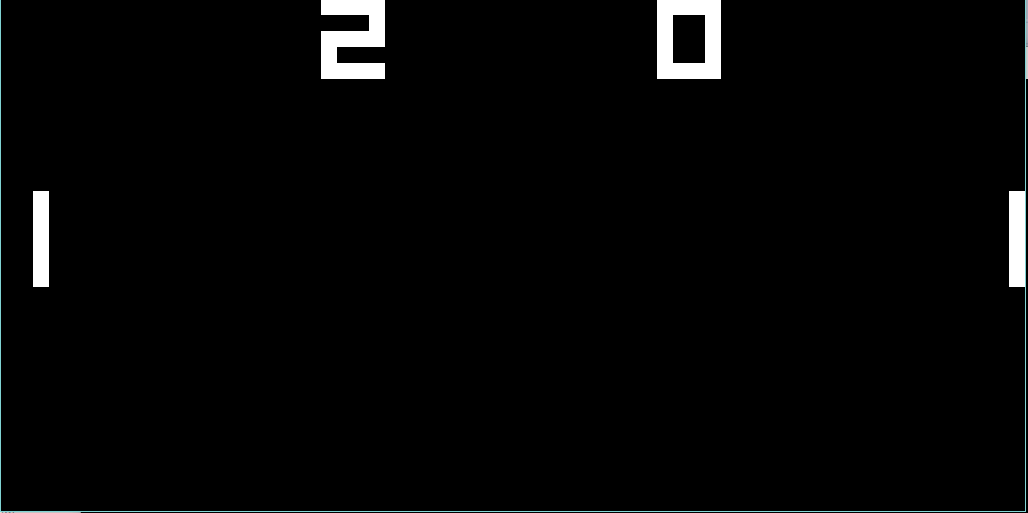
\includegraphics[width=14cm]{chip8cap5.PNG}

\bigskip
\bigskip

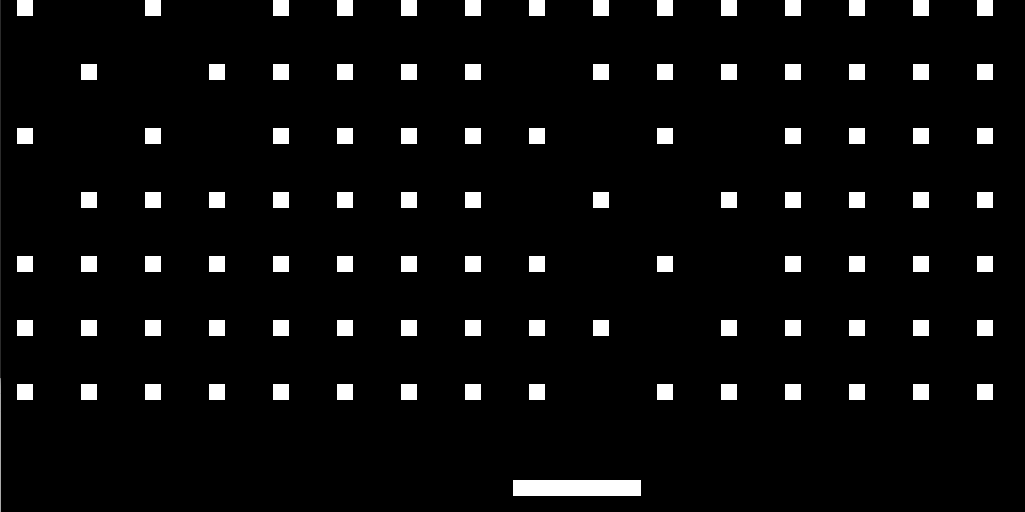
\includegraphics[width=14cm]{chip8cap6.PNG}

\end{document}
